% Principally, this chapter should describe the work which was undertaken before code was written, hardware built or theories worked on. It should show how the project proposal was further refined and clarified, so that the implementation stage could go smoothly rather than by trial and error.

% Throughout this chapter and indeed the whole dissertation, it is essential to demonstrate that a proper professional approach was employed.

% The nature of this chapter will vary greatly from one dissertation to another but, underlining the professional approach, this chapter will very likely include a section headed "Requirements Analysis" and refer to appropriate software engineering techniques used in the dissertation. The chapter will also cite any new programming languages and systems which had to be learnt and will mention complicated theories or algorithms which required understanding.

% It is essential to declare the starting point. This states any existing codebase or materials that your project builds on. The text here can commonly be identical to the text in your proposal, but it may enlarge on it or report variations. For instance, the true starting point may have turned out to be different from that declared in the proposal and such discrepancies must be explained.

% hotstuff algorithm
% why Ocaml - mirage etc.
% chubby (Google) - consensus is hard
% related works

\textit{In this chapter we disclose my knowledge and experience prior to beginning this project [\ref{start}], give a theoretical basis for understanding the HotStuff algorithm [\ref{hotstufftheory}], outline the tools, libraries [\ref{tools}], and methodology [\ref{softwareeng}] deployed in implementation, and highlight the requirements that the implementation should meet [\ref{requirements}].}

\section{Starting point} \label{start}
I had some experience using OCaml from the IA course but had never used it in a project. I also had some background in distributed systems from the IB course, which briefly covered Raft, a non-byzantine consensus algorithm. I had some understanding of byzantine consensus from my own reading into Nakamoto consensus and from developing a wallet application for Ethereum; neither of these was directly useful to implementing HotStuff, but they gave me some wider context of the field.

% the whole implementation was written from scratch??

\section{HotStuff algorithm} \label{hotstufftheory}
A consensus algorithm allows a group of nodes to reach agreement on a log of values under adverse conditions, such as messages being lost, or some nodes being byzantine. In each \textit{view} a leader node proposes some value by sending it the the \textit{replicas} (another word for nodes). After several messages are exchanged the log may be committed, meaning that the log has been agreed upon up to that point and cannot be altered. Once the log is committed up to some point the leader can send `decide' to the replicas; if the log is a list of commands, then the new commands can safely be executed. A consensus algorithm must have these properties:

\begin{itemize}
	\item Safety: Once a log has been committed up to some point that part of the log is immutable, it can only appended to.
	\item Liveness: The system is guaranteed to make progress once a non-faulty leader is elected.
\end{itemize}

The adverse conditions that HotStuff can operate under are described by the system model: partially synchronous, byzantine, with reliable, authenticated, point-to-point delivery. This means that messages sent by one party will always be delivered to another within some bounded amount of time after global synchronisation time (GST) has been reached and a message source cannot be spoofed. The byzantine assumption means a maximum of $f$ faulty nodes may be controlled by an adversary that is actively trying to prevent the nodes from reaching consensus, where $n = 3f + 1$ and $n$ is the total number of nodes.

\subsection{Non-byzantine consensus}
We will start by describing an algorithm to solve the simpler problem of reaching consensus with the stronger assumption of a crash-stop model instead of a byzantine one; this means that we assume nodes cannot be malicious but they can still crash and never come back online. Examples of similar algorithms include Raft and multi-shot Paxos.

Each view can be broken into two phases; phase 1 allows the leader to learn of previously decided values, and in phase 2 it decides on a value. Phase 1 is initiated by the leader broadcasting the current view number to the replicas, which respond by sending their longest accepted log (the one with the highest corresponding view number). Once the leader has a quorum of responses, it initiates phase 2: it selects the longest log that has been sent to it and broadcasts it to the replicas. The leader may also extend the log at this point with its own values, or create a new log if it did not receive anything. Finally, each replica updates its log to the value sent by the leader and sends an acknowledgement. Once the leader receives a quorum of acknowledgements it can commit the new log. This algorithm satisfies our requirement that a committed log can only be extended.

We will refer to phase 1 as the \textit{new-view} stage, and phase 2 as the \textit{commit} phase to use the terminology of the HotStuff paper. These are followed by the \textit{decide} phase, in which the leader sends a decide message to replicas. Once they receive this message they can consider the log decided, and execute the new commands which have been added to the log. See an example in figure \ref{nonbyzantineexample}.
% *** replace with diagrams?
\begin{figure}[h!] 
\texttt{
\begin{enumerate}
\item New-view: 
	\begin{enumerate}
	\item leader $\to$ replicas: ``view = 3" 
	\item replicas $\to$ leader: ``view = 2, log = [`hello', `world']", ...
	\end{enumerate}
\item Commit:
	\begin{enumerate}
	\item leader $\to$ replicas: propose ``log = [`hello', `world', `!']"
	\item replicas $\to$ leader: ``ack", \dots
	\end{enumerate}
\item Decide:
	\begin{enumerate}
	\item leader $\to$ replicas: ``decide"
	\item replicas: execute log
	\end{enumerate}
\end{enumerate}
}
\caption{Non-byzantine example}
\label{nonbyzantineexample}
\end{figure}

\subsection{Byzantine consensus}
In order to extend our algorithm to achieve consensus under a Byzantine threat model we must handle two threats that we will deal with in turn. To do this we must first introduce the concept of a `threshold signature'. Acknowledgements from replicas all contain a signature over the message to prove that they were actually sent by the correct node. The leader can create a threshold signature by combining $n - f$ ack messages' signatures to prove that they really received a quorum of acknowledgements. A collection of a quorum of votes with a threshold signature is known as a `quorum certificate' or `QC'.

\begin{enumerate}
\item Threat: Equivocation --- a faulty leader broadcasts one value to some replicas and a different value to others. For example in the case of a cryptocurrency, this could result in a malicious actor (controlling account X) carrying out a double spend attack, sending ``Account X transfers account Y £10" to some nodes, and ``Account X transfers account Z £10" to other nodes, even if Account X only contains £10.

Solution: Add a new stage \textit{prepare} which happens just before the \textit{commit} phase. In this phase the leader again chooses the longest log it received in the \textit{new-view} phase to pre-propose in the \textit{prepare} phase; the log may also be extended with the leader's new values. Once the leader receives a quorum of acknowledgements, the \textit{commit} phase begins. The difference is that this time the leader includes in its proposal a QC over \textit{prepare} acks, which proves that it pre-proposed the value to at least $n - f$ nodes and received their acks, so it is not proposing one value to some nodes and another value to others.

\item Threat: A faulty leader sends in the \textit{prepare} phase a log that conflicts with one that has already been committed.

Solution: Replicas must \textit{lock} on a value once it is committed and not accept a \textit{prepare} from a leader that contradicts that. They will store the QC that they receive during the \textit{commit} phase and will only accept a new \textit{prepare} if it extends from the node stored in the certificate.
\end{enumerate}

[*** quick inductive proof of hotstuff!] See an example in figure \ref{byzantineexample}.

\begin{figure}[h!] 
\texttt{
\begin{enumerate}
\item New-view: 
	\begin{enumerate}
	\item leader $\to$ replicas: ``view = 3" 
	\item replicas $\to$ leader: ``view = 2, log = [`hello', `world']", \dots
	\item leader: waits $\Delta$ to hear from all non-faulty replicas
	\end{enumerate}
\item Prepare:
	\begin{enumerate}
	\item leader $\to$ replicas: pre-propose ``log = [`hello', `world', `!']"
	\item replicas verify the pre-proposal does not conflict with their \textit{lock}
	\item replicas $\to$ leader: ``log = [`hello', `world', `!'] ack", \dots
	\end{enumerate}
\item Commit (lock):
	\begin{enumerate}
	\item leader $\to$ replicas: propose ``log = [`hello', `world', `!']", qc = (\textit{prepare} acks from previous stage)"
	\item replicas \textit{lock} on the proposed log
	\item replicas $\to$ leader: ``ack", \dots
	\end{enumerate}
\item Decide:
	\begin{enumerate}
	\item leader $\to$ replicas: ``decide, qc = (\textit{commit} acks from previous stage)"
	\item replicas: execute log
	\end{enumerate}
\end{enumerate}
}
\caption{Byzantine example}
\label{byzantineexample}
\end{figure}

% REWRITE THIS SECTION ***
\subsection{Optimistic responsiveness}
A system is responsive if it is able to make progress as fast as conditions allow when a non-faulty leader is elected. If a system must wait for some timeout $\Delta$ to elapse before making progress then it is not responsive.

The algorithm demonstrated in figure \ref{byzantineexample} is not responsive. In the \textit{new-view} phase the leader must wait to hear from $n - f$ replicas, and for a timeout of $\Delta$ to elapse. The timeout is necessary for the system to have the liveness property, so that it can always make progress when a non-faulty leader is elected. Consider again the \textit{prepare} phase; the leader includes in its pre-proposal the QC from the highest view that it hears about in the \textit{new-view} messages it receives. However, there may be some honest replica [how???] that the leader did not hear from (perhaps their message was lost) that is locked on a higher-view proposal than the one that the leader chooses to pre-propose. When this replica receives the pre-proposal, it will reject it as it is locked on a higher-view proposal, and the system will not make progress. This is why it is necessary to wait for a timeout $\Delta$, so that the leader waits a sufficient amount of time to receive a \textit{new-view} from all replicas.

In order to achieve responsiveness we can modify our algorithm by adding a \textit{pre-commit} phase in between \textit{prepare} and \textit{commit}, and removing the requirement for the leader to wait for a timeout in the \textit{new-view} phase. As before, there may be some honest replica that becomes locked on some proposal $x$ during the \textit{commit} phase. However, now there is a \textit{pre-commit} phase before this, where a quorum of replicas all store a \textit{key} for $x$, with this \textit{key} being a QC of \textit{prepare} acks. We now consider the next \textit{new-view} phase; the replicas now send their \textit{key} to the new leader, and the leader chooses what to propose based on the highest view \textit{key} it sees. Even if the leader does not receive a \textit{new-view} from the honest replica itself, it is guaranteed to hear about the proposal $x$, so it will be able to make progress. See an example in figure \ref{responsiveeexample}.

% This ensures that if some honest replica becomes locked on a value in the \textit{commit} phase, then there are at least $f + 1$ honest nodes that have a `key' for that value from the \textit{pre-commit} phase. More specifically, they have a `key-proof' composed of a QC over \textit{pre-commit} acks. Replicas then send this key-proof with their \textit{new-view} message when a new view begins. The new leader selects the key-proof with the highest view proposal and sends it along with their \textit{prepare} message. Even if the leader does not receive a \textit{new-view} message from the replica that is locked on the highest view proposal, they must have received the key to this proposal from some honest replica, so their \textit{prepare} message will make progress. See an example in figure \ref{responsiveeexample}.

\begin{figure}[h!]
\texttt{
\begin{enumerate}
\item New view: 
	\begin{enumerate}
	\item leader $\to$ replicas: ``view = 3" 
	\item replicas $\to$ leader: ``qc = (\textit{key} for view = 2, log = [`hello', `world'])", \dots
	\end{enumerate}
\item Prepare:
	\begin{enumerate}
	\item leader $\to$ replicas: pre-propose ``log = [`hello', `world', `!'], qc = (key for view = 2, log = [`hello', `world'])"
	\item replicas verify the pre-proposal does not conflict with their \textit{lock}
	\item replicas $\to$ leader: ``log = [`hello', `world', `!'] ack", \dots
	\end{enumerate}
\item Pre-commit (key):
	\begin{enumerate}
	\item leader $\to$ replicas: ``qc = (\textit{prepare} acks from previous stage)"
	\item replicas store qc as a \textit{key}
	\item replicas $\to$ leader: ``log = [`hello', `world', `!'] ack", \dots
	\end{enumerate}
\item Commit (lock):
	\begin{enumerate}
	\item leader $\to$ replicas: propose ``qc = (\textit{pre-commit} acks from previous stage)"
	\item replicas \textit{lock} on proposed log
	\item replicas $\to$ leader: ``ack", \dots
	\end{enumerate}
\item Decide:
	\begin{enumerate}
	\item leader $\to$ replicas: ``decide, qc = (\textit{commit} acks from previous stage)"
	\item replicas: execute log
	\end{enumerate}
\end{enumerate}
}
\caption{Responsive example}
\label{responsiveeexample}
\end{figure}

\subsection{View-changes} \label{viewchange}
If a leader fails to make progress within some timeout a view-change takes place and the next view begins. The HotStuff paper does not go into detail on how view-changes take place, so this explanation is based on a talk by one of its authors, Ittai Abraham \cite{ittai}.

Once the view times out, nodes send a \textit{complain} message to the next leader and start a new timeout for the next view. Once the next leader achieves a quorum of \textit{complain} messages it collects them into a QC known as a \textit{view-change proof}. This leader can then send a \textit{view-change} message containing the \textit{view-change proof} to all replicas, who will respond by transitioning to the next view and sending a \textit{new-view} message to the new leader. The inclusion of the \textit{view-change proof} prevents liveness attacks by byzantine nodes that could otherwise attack the system by constantly causing view-changes to take place and preventing non-faulty leaders from making progress.

The use of timeouts in this way is a type of failure detector, which is a system that facilitates the detection of failed nodes. [add more information on failure detectors ***]

\subsection{Chaining} \label{chaining}
The algorithm presented goes through several very similar phases to commit a proposal, these phases involve collecting votes from replicas to form a QC that then serves in later phases. The `chained' algorithm simplifies and optimises this by pipelining the different phases. Instead of having different phases as before, we can have a single \textit{generic} phase that collects votes, creates a \textit{generic QC}, and sends it to the next leader; now we change view on each phase and a QC can serve in multiple phases concurrently.

In each view, some leader sends a proposal to all replicas, who send their replies to the next leader who can form a QC to add to their proposal. The replicas also send \textit{new-view} messages to the next leader as before, to allow them to select a node to propose.

\begin{figure}[h!]
\centering
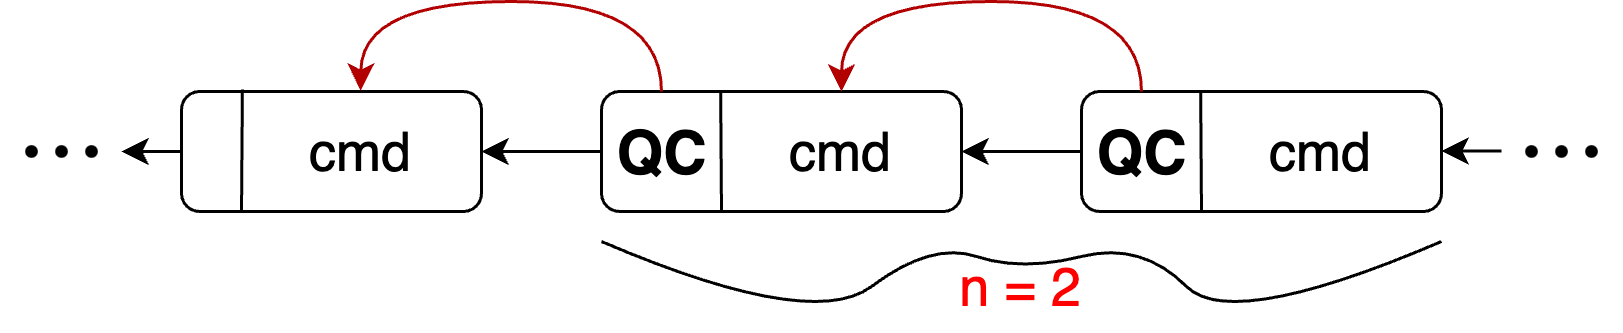
\includegraphics[scale=0.3]{nchain.png}
\label{nchain}
\end{figure}

Figure \ref{nchain} shows a chain of nodes connected by `parent' links; every time we propose a value we extend the chain with a new node. Some node \textit{b} also contains a link to another node within \textit{b.justify.node}, which is the previous generic QC in the chain. In the event of a view-change a dummy node will be inserted in the chain which will cause a `gap' where some \textit{b.justify.node} pointer jumps over a dummy node. If some node \textit{b} has a QC that points to its direct parent with no `gap' in-between, then we say that it forms a \textit{one-chain}. In general, if we have $n$ such direct links without `gaps' we refer to this as an \textit{n-chain}, as shown above.

To reproduce the behaviour of the unchained algorithm, on receiving a proposal for node \textit{b\textsuperscript{*}} a replica must look at \textit{b\textsuperscript{*}.justify.node} to see if it points to an \textit{n-chain}. It must take different actions depending on the length of the chain:

\begin{itemize}
\item zero-chain: this is equivalent to the \textit{prepare} phase from the unchained version, so the replica votes for the proposal only if it does not conflict with their \textit{lock}
\item one-chain: this is equivalent to the \textit{pre-commit} phase from the unchained version, so the replica should store a \textit{key}
\item two-chain: this is equivalent to the \textit{commit} phase, so the replica should \textit{lock} on the value proposed at the start of the two-chain
\item three-chain: this is equivalent to the \textit{decide} phase, so the replica can execute the commands from the node at the start of the three-chain
\end{itemize}

\section{Tools \& libraries} \label{tools}
\textit{In this section we outline the languages and libraries used in implementation, and justify why they were appropriate for this project.}

\subsection{OCaml}
I chose OCaml for this project due to its high-level nature, static type system, ability to blend functional and imperative paradigms, and good library support. OCaml's multi-paradigm nature is suitable for implementing HotStuff, as the core state machine can be elegantly expressed in a functional way, whereas interacting with the RPC library to send messages is better suited to an imperative paradigm. Additionally, the Tezos cryptocurrency is written in OCaml and contains a cryptography library that provides the functionality needed by HotStuff.

The performance bottlenecks for distributed byzantine algorithms are generally cryptography, message serialisation and network delays. This means that it is more important to choose a language with suitable features to aid implementation, rather than picking a `high-performance' language like C++.

OCaml has a powerful module system that facilitates writing highly reusable code. The module system was only briefly touched upon in the tripos (in Concepts in Programming Languages from IB), so I spent time learning about these features. Modules provide an elegant interface for the core state machine to interact with the imperative parts of the program that actually send messages over the network.

There is no existing reference implementation of HotStuff in OCaml, so my project contributes to the growing OCaml ecosystem. This ecosystem is home to an active community, and interesting projects such as MirageOS unikernels. Because my project is implemented purely in OCaml, it could potentially be deployed on a MirageOS unikernel [???].

\subsection{Lwt}
Lwt is a concurrent programming library for OCaml. It allows the creation of promises, which are values that will become determined in the future; these promises may spawn threads that perform computation and I/O in parallel. In order to use Lwt I had to learn about monads, which are ways of sequencing effects in functional languages and are used by asynchronous promises in Lwt. Lwt is useful to this project as promises provide a way to dispatch messages over the network and wait for their responses in different threads. Promises are cheap to create in Lwt, so one can create many lightweight threads with good performance [citation needed***].

One alternative I could have used is Jane Street's Async library [citation needed???], which has similar features but better performance. I chose not to use this library due to its poor documentation. Another alternative that has better performance than Lwt is EIO [citation needed???], but this library is new and not yet in a stable state.

\subsection{Cap'n Proto}
Cap'n Proto is an RPC framework that includes a library for sending and receiving RPCs, and a schema language for designing the format of RPCs that can be sent. Benchmarks for the library are presented in \ref{capnpbenchmark}.

\subsection{Tezos cryptography} \label{tezos}
The Tezos cryptography library provides aggregate signatures using the BLS12-381 elliptic curve construction. It provides functions to sign some data using a private key, aggregate several signatures into a single one, and check whether an aggregate signature is valid. The only difference from the threshold signatures needed by HotStuff is that each individual signature in an aggregate signature can sign different data, whereas with threshold signatures each individual signature is over the same data. It is trivial to implement threshold signatures using this library by checking that the data is the same for all signatures inside the aggregate signature. Benchmarks for the library are presented in section \ref{tezosbenchmark}.

\section{Requirements analysis} \label{requirements}

In order to be successful the implementation should conform to the following requirements:

\begin{itemize}
	\item Correctness --- the consensus algorithm should be implemented as it is described in the paper \ref{hotstuff}. This can be established by testing the program trace for compliance with the algorithm specification [do I need to mention change from proposal here ***].
	\item Evaluation --- analysis of system throughput and latency should be carried out on a simulated network of 4 replicas. Evaluation will be carried out by testing the program locally, analysing the trace, and testing in an emulator.
	\item Improve transaction throughput and reduce latency [compared to what? ***]. This can be achieved through architectural decisions, tuning the scheduler, and ensuring cryptographic libraries are being used efficiently.
	% \item Description of how to implement verifiable anonymous identities on top of the HotStuff implementation.
\end{itemize}

These requirements are similar to those presented in my proposal (Appendix X***) with a few differences. The first difference is to evaluate on 4 nodes rather than 32. Benchmarking of Cap'n Proto has revealed its limitations when sending large messages (\ref{capnpbenchmark}). Once batching of requests is implemented the internal messages sent between nodes will be large and could cause a performance bottleneck for the state machine progressing. Because of this, it may not be feasible to get reasonable performance with more nodes, as more nodes result in more internal messages being sent. In practice, permissioned blockchains are often run with a small number of nodes, so this limitation may not be important [citation needed *** honeybadger BFT?].
% https://github.com/heidihoward/distributed-consensus-reading-list#bft-surveys

% Additionally the extension has been changed from adding support for network reconfiguration to describing how to implement verifiable anonymous identities. This is because this extension seemed like a more interesting direction for the project with more exciting applications.
% mention how the reconfig extension was dropped for focusing on performance improvements

\section{Software engineering practices} \label{softwareeng}

\textit{In this section we describe the professional software engineering methodology deployed during implementation.}

\subsection{Development methodology}
[should i say i used something like RAD and productivity tracking tools???]
\subsection{Testing \& debugging methodology} \label{testing}
Unit testing was carried out using `expect tests', which compare a program trace to the correct output. A testing suite of expect tests verifies that the program behaves as specified in the HotStuff paper. This suite has 100\% code coverage\footnote{The report says 97.89\% coverage, but the only uncovered code is the testing code itself.} of the consensus state machine code, the coverage report is at \textit{\_coverage/index.html}.

The Memtrace library and viewer were used to profile the memory usage of the program. One can generate a flame graph of memory allocations to see which parts of the program are using the most memory.

% mention mininet for evaluation?

Due to the distributed nature of the program, normal debugging tools and profilers are not useful for debugging deadlocks and performance issues. This is because the cause of deadlocks and performance issues is often some process waiting or a backlog of work forming, but this cannot be detected by tools that just track things like CPU usage. Instead, I had to rely on manual inspection of the program trace and commands that measure the real time taken for some part of the program to run.

[implement CI???]
\subsection{Source code management}
I used Git for version control and regularly pushed my local changes to a private GitHub repository.